%!TEX root = ../thesis_a4.tex
\chapter{Implementing User-Tailored Concatenative Synthesis Systems for Electronic Music}
\label{chap:rhythmcat}

%\section{Interfaces and Frameworks for Computer Music}
%
%\subsection{Hardware Interfaces for Electronic Music Production}
%
%\subsection{Software Interfaces for Electronic Music Production}
%
%\subsection{Digital Audio Workstations}
%
%\subsubsection{Timeline Interfaces}
%
%\subsubsection{Non-linear Interfaces}
%
%For live and real-time electronic music linear audio software systems are desirable neither by performers nor audiences. Of course experimental music practicioners have been devising their own boutique software interfaces for realising public performance. Adventurous early dance music producers like Modeselektor and Apparat also built primitive "looper 
%
%\subsection{Software Instrument Interfaces}

\section{Introduction}

\chapref{chap:pyconcat} offered a deep, technical description and implementation of key methods in concatenative synthesis culminating in the proposal of some novel contributions that we hope advances the state of the art in a meaningful and valuable manner. This chapter, on the other hand, is all about the \textit{practical} aspects of adapting concatenative synthesis for everyday integration into the workflows of our target user - the dance music producer. The two biggest challenges we face here can be distilled to:

\begin{enumerate}
  \item \textit{Interface} - devising appealing and visualisation strategies and interaction metaphors for communicating gesture and feedback
  \item \textit{Performance} - striking a balance between accuracy and feasibility 
\end{enumerate}


\section{Visualising and Interacting with Sound}

Up until now the conversation with our synthesis engine has been abstract and textual. Content is fed to the system, some parameters are set and the patient user, after a time, receives the rendered output. For many users\footnote{And computer music composers of a certain vintage.} and their musical applications, this is perfectly acceptable way of creating sounds. For many other users, and we mean here dance music producers who are used to a wide range of user friendly and appealing music interfaces, it is clearly not an ideal \textit{metaphor} for visualising their sound or interacting with them. 

Metaphor, in the context of human computer interaction and the craft of designing interfaces can  

\paragraph{The Waveform Metaphor}

\paragraph{The Loop Grid Metaphor}

\paragraph{The Modular Metaphor}


Visualising sound and music coherently, in a meaningful yer pleasing manner is and, more importantly analytical representations is an ongoing challenge that faces all music information researchers.

In CataRT \citep{Schwarz2006a}, timbreID \cite{Brent2010} and earGram \citep{Bernardes2013} for example, the sounds are position in a timbre space by assigning a specific feature (or dimension of a vector feature) to each axis, with a third dimension assigned to RGB colour scale \footnote{Though Bernardes does extend the option for  dimensionality reduction using Star Coordinates \citep{Cooprider2007}, a technique based on summing the feature vectors.}. This is particularly useful in the case of scalar features with a very coherent perceptual correspondence.  In \figref{fig:temporal_and_spectral_features} we see a plot of every combination of temporal and spectral features used in the classification in \chapref{chap:pyconcat} . Assigning loudness and spectral centroid (or ``brightness'' to give it some perceptual labelling), for instance, presents a meaningful organisation of sounds in 2D timbre space (top-right in the figure) and are easily comprehensible by the lay user. But choosing only two features from a rich set of descriptors in multidimensional timbre space can discard potentially important statistics that can give good separation between points. Furthermore, while loudness and ``brightness'' are lucid qualities for many users, expecting them to compare and decipher higher order cepstral coefficients is perhaps not so transparent.

\begin{figure}
	\begin{center}
		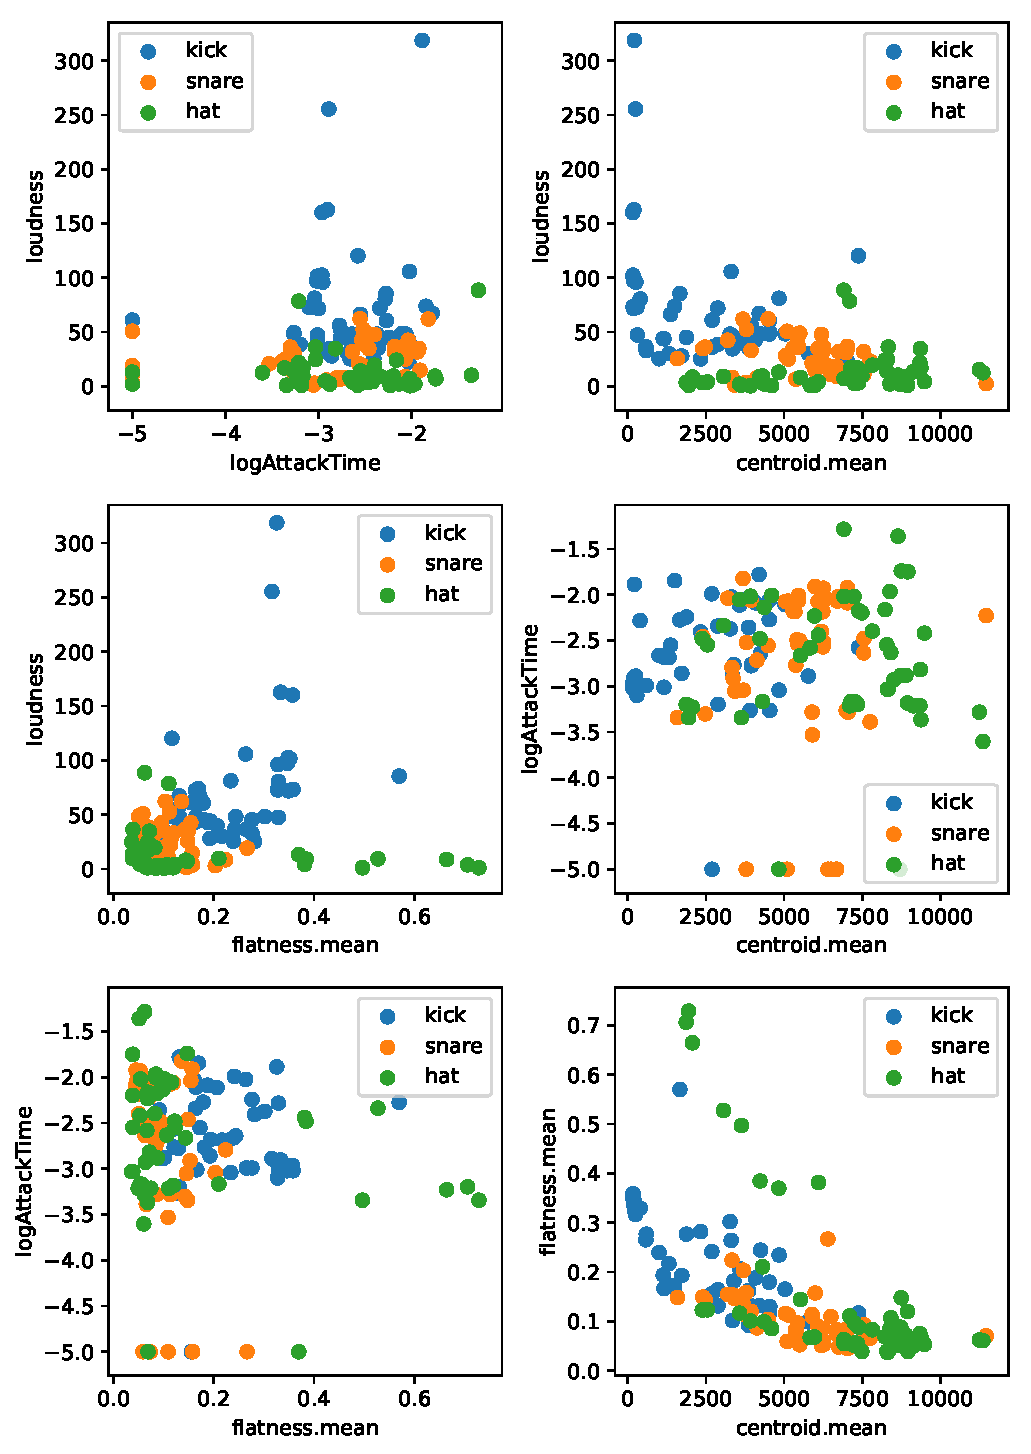
\includegraphics[width=1.0\textwidth]{ch06_rhythmcat/figures/feature_axis_combos.pdf}
	\end{center}
	\caption[Visualisation of all temporal and spectral feature combinations for kick, snare and hat drum sounds]{Visualisation of all temporal and spectral (taking the mean only) feature combinations for kick, snare and hat drum sounds}
	\label{fig:temporal_and_spectral_features}
\end{figure}

\subsection{Timbre Spaces and Dimensionality Reduction Techniques}

To address some of the shortcomings of visualisation based on raw singular feature values, it is often useful to apply a formal dimensionality reduction technique that can provide an `automatic' projection of the higher-order feature space into a so-called timbre space (created with a scatter plot) suitable for visualisation of the data, while hopefully retaining most of the important trends latent within the data. So-called ``timbre spaces''  have been talked about in the literature for quite some time, but one of the key innovators in the usage of timbre spaces for creative or generative purposes has been David Wessel. By taking measurements of subjective responses to timbral stimuli, dimensionality reduction schemes are used to present a map of timbral references in space that can be then used to provide a spatial reference for generation and control of additive synthesis \citep{Wessel1979, Wessel1976}

Specifically in the context of organising and exploring multimedia collections based on similarity, Christian Frisson's doctoral thesis \citeyearpar{frisson2015} offers a broad and up-to-date introduction to the main techniques and is worthwhile reference.

\paragraph{Principal Component Analysis}

\acrfull{pca} is a statistical procedure applied to data that can discover trends in order to preserve those with the most variance, effectively allowing us to compress data from high-dimensional space into lower-dimensional space without considerable ``loss'' of salience \cite{Hackeling2014} . Practical applications of \acrshort{pca} includes reducing redundant (features with low variance) data for more efficient machine learning tasks, and for producing coordinates that can make comparative visualisation of data possible in 2 or 3 dimensions.

It is the second application that interests us here, and in fact \acrshort{pca} has seen considerable application already in visualisation for musical applications \citep{Cooper2006}. Most of these involve organising large musical collections, . Within the GiantSteps project, or colleagues have compared  \acrshort{pca} with \acrshort{mds} (see below) 

\acrshort{pca} involves a few stages of matrix algebra and is implemented already in many libraries and frameworks so we won't dwell on it too heavily here. However the key stages are summarised in an excellent tutorial by \citep{Smith2002a}. Basically, the method uses eigenvalues and eigenvectors to extract the axes of maximum variance from the covariance matrix of the original data, and the highest eigenvectors are the principal components. As many principal components can be retained as required, with the assumption being that the loss will be minimal as more components are discarded.

\paragraph{Multidimensional Scaling}

\acrfull{mds} actually refers to a taxonomy of methods for dimensional reductions including `classical' or \acrfull{pcoa}, metric and non-metric \acrshort{mds}. \acrshort{mds} uses a distance or dissimilarity matrix as input and attempts to reduce the dimensions while preserving pairwise distance between entities, compared to \acrshort{pca} which tries to preserve maximum variance (or as \cite{frisson2015} puts it more succintly: ``\acrshort{mds} uses a distance matrix whereas \acrshort{pca} uses a correlation matrix.'')

Regarding musical applications, \acrshort{mds} has been used somewhat less that \acrshort{pca}. Within the GiantSteps project, our colleagues have been studying the effects of symbolic rhythmic features on the organisation of symbolic rhythmic patterns in dance music when dimensionality reduction techniques such as \acrshort{pca}, \acrshort{mds} and \acrshort{tsne} (to follow) are applied. This buildings on previous perceptual dimensional scaling studies conducted by Gabrielson in the 1970s. 

\paragraph{t-Distributed Stochastic Neighbour Embedding}

\acrfull{tsne} is a relatively recent award-winning approach to data visualisation that is tailored specifically for effective reduction of high-dimensional datasets \citep{VanDerMaaten2008}. Based on a previous method known as \acrfull{sne}, one of improvements it offers is  reductional strategies for preventing crowding or over-layered clusters in the centre of the map inherent in \acrshort{sne} methods. Essentially this is achieved by using a Student-t distribution rather than Gaussian for computing dissimilarity between points in low-dimensional space \citep{VanDerMaaten2008}	.

The \acrshort{tsne} algorithm is gaining considerable favour in music information tasks as a way of navigating large collections of complex data representations. 

In a comparative evaluation of \acrshort{mds}, \acrshort{pca} and \acrshort{tsne} based on three criteria \citep{Dupont2013} reveals that t-SNE outranks PCA which in turn outranks \acrshort{mds} in three tasks related to musical loops and sound effects.

Returning to our own tasks of visualising feature vectors of drum sounds, \figref{fig:dimension_reductions} shows these three dimension reduction techniques applied to 50 instances each of kick, snare and hi-hat sounds based on the full gamut of features extrapolated with the GFCC+Spectral+Temporal configuration. One thing that's immediately apparent across all methods is their increased used of the 2-dimensional space in comparison to the individual assignment of features to axes as we saw in \figref{fig:temporal_and_spectral_features}, as well as exhibiting less crowding in overlapping clusters.

Most methods are quite capable of sorting the distinctive low frequency membrane kick sounds from the snares and hi-hats which are both b

\begin{figure}
	\begin{center}
		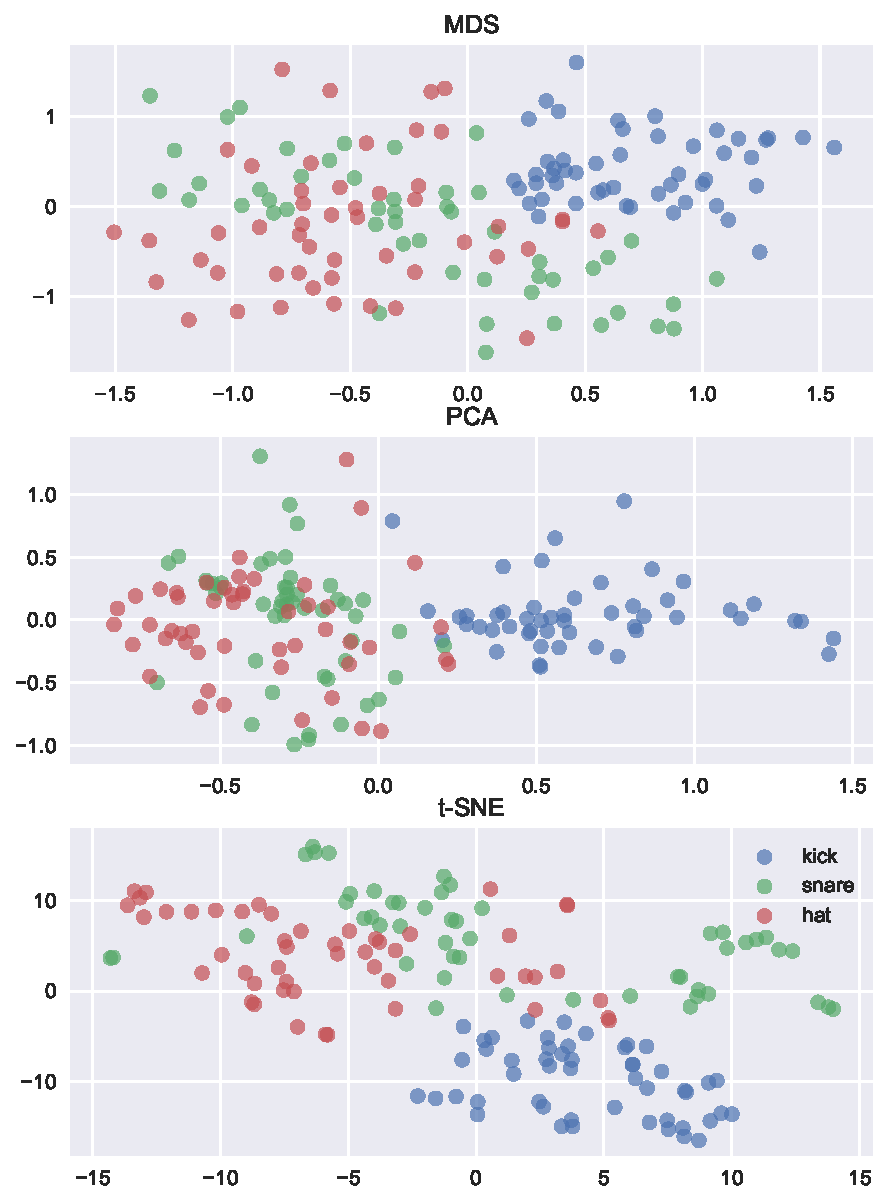
\includegraphics[width=1.0\textwidth]{ch06_rhythmcat/figures/dimension_reductions.pdf}
	\end{center}
	\caption[MDS, PCA and t-SNE Dimension Reduction on Kick,Snare and Hat Sounds]{\acrshort{mds}, \acrshort{pca} and \acrshort{tsne} dimension reduction processes applied to kick, snare and hi-hat sounds}
	\label{fig:dimension_reductions}
\end{figure}

\subsubsection{Interacting with Sounds and Creating a Metaphor}

Undoubtably, the timbre space paradigm represent a much richer modality for organising sound spatially and a provides a vital window into the procedures governing concatenative synthesis. We have seen how exactly rendering these spaces is not trivial and poses a unique set of challenges and tradeoffs to get a usable and meaningful landscape for exploration.

Equally challenging once a timbre space has organised a visual map of sound is how to \textit{interact} with those sounds. How can the user effectively navigate this sonic terrain and avail of suitable gesture and metaphor to arrange the sounds in the desired manner? How do existing concatenative synthesis deal with these challenges? To complicate matters further, our system is inherently rhythm driven. How do those sound exploratory devices extend to our unique problem domain?

In CataRT the primary interaction metaphor is simple and intuitive: the target is the real-time position of the mouse cursor and a resizable radar around the target filters the range of sounds within its proximity. How these sounds are triggered depends on the mode selected. The triggering modes include:

\begin{itemize}
  \item \textit{Bow} - trigger closest unit each time you move the mouse
  \item \textit{Fence} - like a stick dragging along a fence, triggers when a new unit becomes closer to the target
  \item \textit{Beat} - triggers according to metronome
  \item \textit{Chain} - triggers after previous unit finishes
  \item \textit{Quant} - non-functional quantised mode
  \item \textit{Seq} - trigger via external sequencer
  \item \textit{Cont} - play back units in order
\end{itemize}

In earGram the SpaceMap mode also triggers units based on proximity to the mouse pointer target, but defines three different triggering modes distinct from CataRT:

 \begin{itemize}
  \item \textit{continuousPointer} - continuously play units at a specified rate
  \item \textit{pointerClick} - same as continuousPointer but ``played in response to a controller command'' (the meaning of this is not exactly clear from the description provided)
  \item \textit{colorPicker} - selects units based on a colours 
  \item \textit{liveInput} - feature analysis of live input sets pointer position
\end{itemize} 

AudioGarden appears to adapt the mouse radar approach of CataRT also, but also the positioning of multiple radars in the timbre space that can trigger multiple grains for a single unit in time which is a very simple and useful method of mixing corpus units.

\begin{figure}
	\begin{center}
		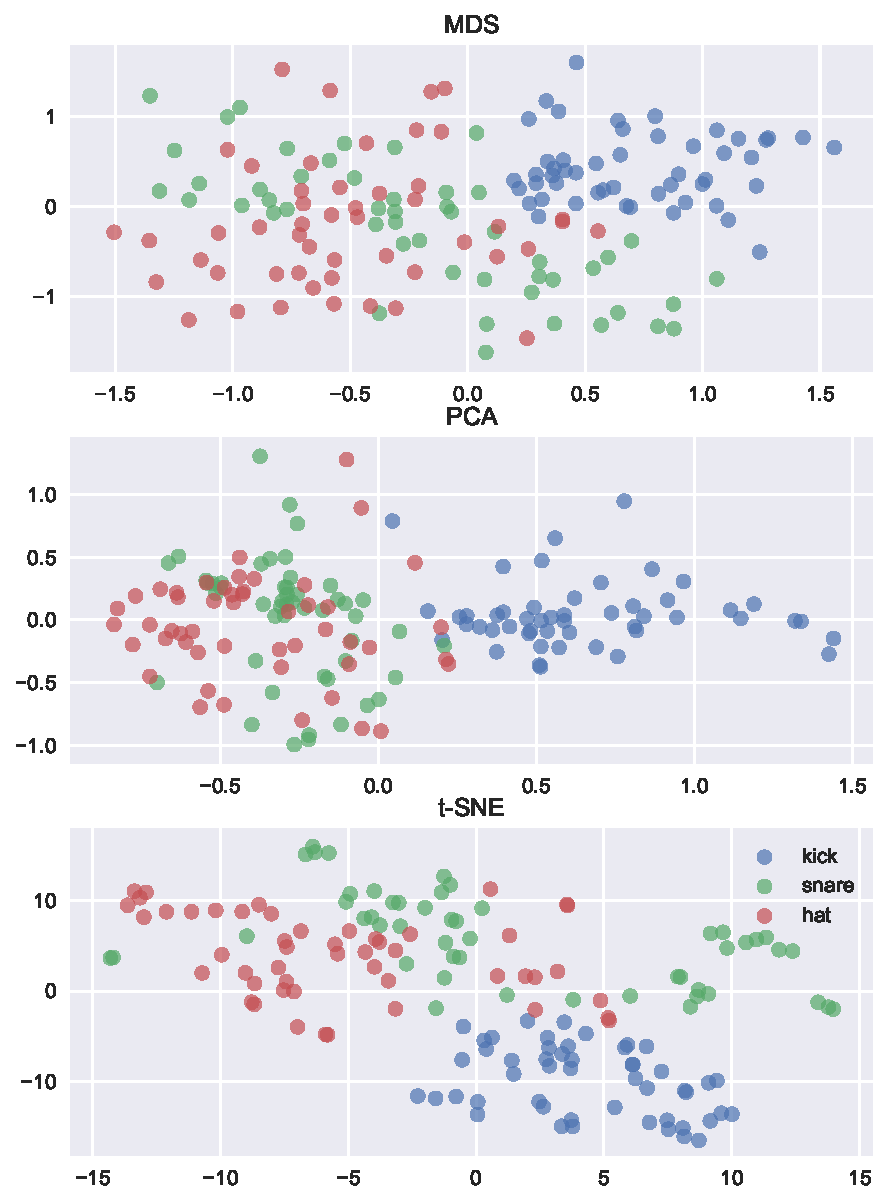
\includegraphics[width=1.0\textwidth]{ch06_rhythmcat/figures/dimension_reductions.pdf}
	\end{center}
	\caption[MDS, PCA and t-SNE Dimension Reduction on Kick,Snare and Hat Sounds]{\acrshort{mds}, \acrshort{pca} and \acrshort{tsne} dimension reduction processes applied to kick, snare and hi-hat sounds}
	\label{fig:dimension_reductions}
\end{figure}

\section{RhythmCAT}

\subsection{Identifying our Users}

<TODO - TALK ABOUT MUSIC PRODUCERS, RED BULL ETC>

\subsection{Real-time Challenges}

<TODO - EXPLAIN CHALLENGES WITH HMM AND REAL-TIME>

\subsection{Developing the System}

In this section, we will describe our implementation of the RhythmCAT system, beginning with an explanation of the musical analysis stages of onset detection, segmentation and feature extraction. This is followed by an examination of the interactive user interface and the pattern generation process. Figure 1 gives a diagrammatic overview of these important stages, which can be briefly summarised as:

\begin{enumerate}
  \item Sound Input
  \item Onset Detection \& Segmentation
  \item Audio Feature Extraction
  \item Storage \& Data Representation
  \item Pattern Synthesis
  \item Real-time Audio Output
\end{enumerate}


The system is developed in C++ using the JUCE framework[32], the Essentia musical analysis library \citep{Bogdanov2013} and the OpenCV computer vision library \citep{Bradski2000} (for matrix operations).
 
\subsubsection{Sound Input}

The first stage in building a concatenative music system generally involves gathering a database of sounds to select from during the synthesis procedure. This database can be manually assembled but in many musical cases the starting point is some user-provided audio that may range in length from individual notes to phrases to complete audio tracks.

\begin{figure}
	\begin{center}
		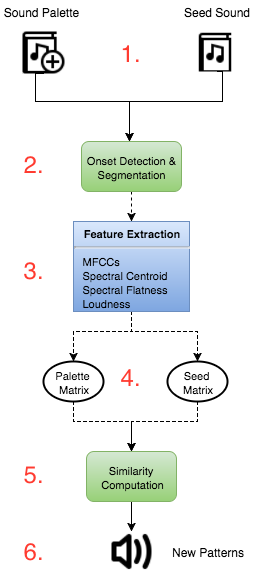
\includegraphics[width=0.5\textwidth]{ch05_pyconcat/figures/rhythmcat_flowchart.png}
	\end{center}
	\caption[Block Diagram of Functionality in RhythmCAT System]{Block Diagram of Functionality in RhythmCAT System}
	\label{fig:rhythmcat_flowchart}
\end{figure}
 
The two inputs to the system are the Sound Palette and the Seed Sound. The sound palette refers to the pool of sound files we want to use as the sample library for generating our new sounds. The seed sound refers to the short loop that we wish to use as the similarity target for generating those sounds. The final output sound is a short (one to two bars) loop of concatenated audio that is rendered in real time to the audio host.

\subsubsection{Onset Detection and Segmentation}

In cases where the sounds destined for the sound palette exceed note or unit length, the audio needs to be split into its constituent units using onset detection and segmentation.
Onset detection is a large topic of continuous study, and we would encourage the reader to examine the excellent review of methods summarised in \citep{Dixon2006}. Currently, with some tuning of the parameters, Sebastien Bock’s Superflux algorithm represents one of the best performing state of the art detection methods \citep{Bock2013}. For our purposes, we have experienced good results with the standard onset detector available in Essentia, which uses two methods based on analysing signal spectra from frame to frame (at a rate of around 11 ms). The first method involves estimating the high-frequency content in each frame
\citep{Masri1996} while the second method involves estimating the differences of phase and magnitude between each frame \citep{Bello2005}.

The onset detection process produces a list of onset times for each audio file, which we use to segment into new audio files corresponding to unit sounds for our concatenative database.

\subsubsection{Audio Feature Extraction}

In music information retrieval systems, the task of deciding which features are used to represent musical and acoustic properties is a crucial one. It is a tradeoff in choosing the richest set of features capable of describing the signal succinctly at the expense of storage and computational complexity. When dealing with musical signals specifically, there are a number of standard features that correspond roughly to certain perceptual sensations. We briefly describe our chosen features here, but for a more thorough treatment of feature selection with relation to percussion the reader should consult \citep{Herrera2003, Roy2007b, Tindale2004, Tindale2004a}.

Our first feature is the loudness of the signal, which is implemented in Essentia according to Steven’s Power Law, namely the energy of the signal raised to the power of 0.67 \citep{Bogdanov2013}. This is purported to be a more perceptually effective measure for human ears. Next we extract the spectral centroid, which is defined as the weighted mean of the spectral bins extracted using the Fourier Transform. Each bin is then weighted by its magnitude.

Perceptually speaking, the spectral centroid relates mostly to the impression of the brightness of a signal. In terms of percussive sounds, one would expect the energy of a kick drum to be more concentrated in the lower end of the spectrum and hence have a lower centroid than that from a snare or crash cymbal.

Another useful single-valued spectral feature is the spectral flatness. It is defined as the geometric mean of the spectrum divided by the arithmetic mean of the spectrum. A spectral flatness value of 1.0 means the energy spectrum is flat whereas a value of 0.0 would suggest spikes in the spectrum indicating harmonic (with a specific frequency) tones. The value intuitively implies a discrimination between noisy or inharmonic signals and harmonic or more tonal signals. Kick drum sounds (especially those generated electronically) often comprise quite a discernible centre frequency whereas snares and cymbals are increasingly broadband in spectral energy.

Our final feature is the vector quality known as \acrshort{mfcc}s (Mel Frequency Cepstrum Coefficients). \acrshort{mfcc}s can be considered as a compact approximation of the spectral envelope that is a useful aid in computationally describing and classifying the “timbre” of a signal. It has been applied extensively in speech processing, genre detection \citep{Tzanetakis2001} and instrument identification \citep{Loughran2004}. \acrshort{mfcc} computation, as outlined in \citep{Logan2000}}, is basically achieved by computing the spectrum, mapping the result into the more perceptually relevant Mel scale, taking the log, then applying the Discrete Cosine Transform.

It is difficult to interpret exactly what each of the \acrshort{mfcc} components mean, but the first component is generally regarded as encapsulating the energy. Since we are already extracting the loudness using another measure we have discarded this component in our system. For detailed explanations and formulae pertaining to the features introduced here as well as others we direct the user to \citep{Peeters2004b}.

\subsubsection{Pattern Synthesis and User Interaction}

Further on in the article we will describe a bit more on how the seed or target audio signal is actually received from the \acrfull{vst} host, but in terms of analysis on that seed signal, the process is the same as before: onset detection and segmentation followed by feature extraction.

The resulting feature vectors are stored in two matrices: the palette matrix and the target matrix. The palette matrix stores the feature vectors of each unit of sound extracted from the sound palette and similarly the target matrix stores feature vectors of units of sound extracted from the seed loop.



\subsubsection{Pattern Synthesis}

This section details the visible, aural and interactive elements of the system as they pertain to the user. Figure 2 gives a glimpse of the user interface in a typical pattern generation scenario.

\paragraph{Workflow}

The layout of the interface was the result of a number of iterations of testing with users who, while praising the novelty and sonic value of the instrument, sometimes expressed difficulty understanding the operation of the system. One of the main challenges faced was how best to present to the user the general workflow in a simple and concise manner. It was decided to represent the flow of the various operations of the software emphatically by using a simple set of icons and arrows, as is visible in Figure 2 - A.

\begin{figure}
	\begin{center}
		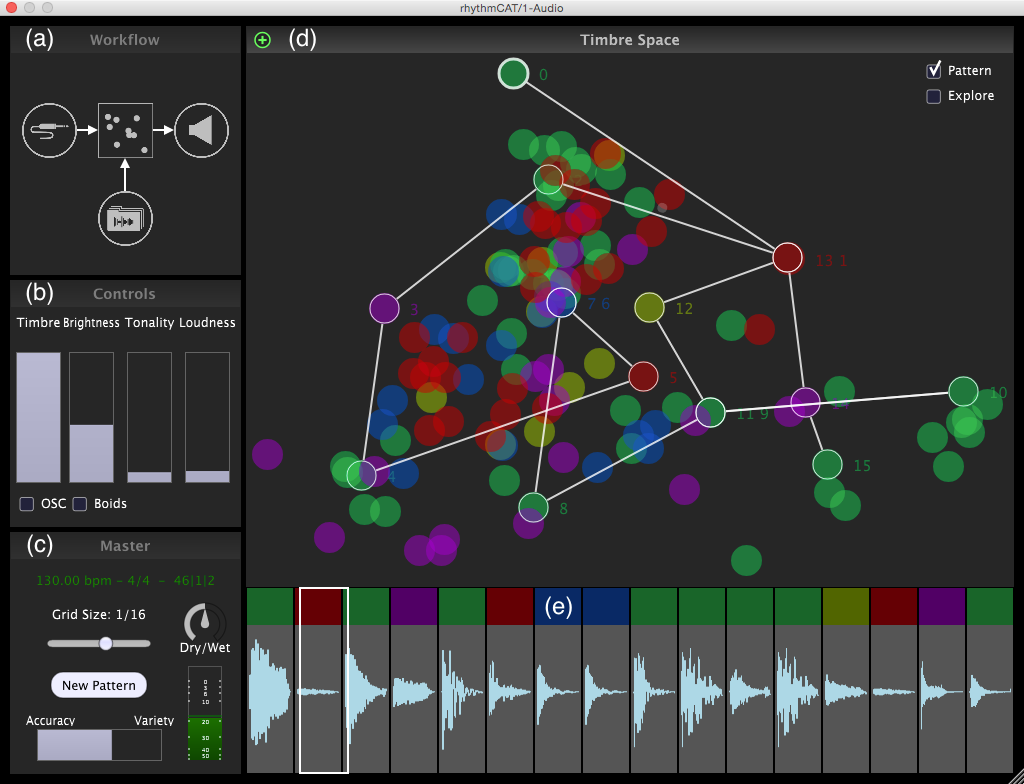
\includegraphics[width=1.0\textwidth]{ch05_pyconcat/figures/rhythmcat.png}
	\end{center}
	\caption[Main User Interface Showing Panels A-E with Onset Graph]{Main User Interface Showing Panels A-E with Onset Graph}
	\label{fig:rhythmcat_interface}
\end{figure}
 
The icons indicate the four main logical operations that the user is likely to do, and opens up the related dialogs, namely:
\begin{itemize}
  \item The Palette Dialog - as indicated by the folder icon
  \item The Seed Dialog - as indicated by the jack cable icon
  \item The Sonic Dialog - as indicated by the square feature space icon
  \item The Output Dialog - as indicated by the speaker icon
\end{itemize}

\paragraph{Sound Palette}

The user loads a selection of audio files or, folders containing audio files, which are analysed to create the sound palette as has previously been discussed. Next, dimensionality reduction is performed on each feature vector of the units in the sound palette using \acrfull{pca}. Two \acrshort{pca} components are retained and scaled to the visible area of the interface to serve as coordinates for placing a circular representation of the sound in two-dimensional space. These visual representations, along with their associated audio content, we term sound objects. They are clearly visible in main timbre space window in the figure.

\paragraph{Seed Input}

Seed audio is captured and analysed by recording directly from the input audio of the track on which the instrument resides in the audio host. Using the real-time tempo and bar/beat information provided by the host, the recorder will wait until the next bar starts to begin capture, and will only capture complete bars of audio. This audio is analysed as before but with one exception. Since the goal of the instrument is to integrate with an existing session and generate looped material, we make the assumption that the incoming audio is quantised and matches the tempo of the session. Thus, onset detection is not performed on the seed input; rather, segmentation takes place at the points in time determined by the grid size (lower left of the screen).

An important aspect to note: since the instrument is fundamentally real-time in its operation, we need to be careful about performing potentially time consuming operations such as feature extraction when the audio system is running. Thus, we perform the audio recording stage and feature extraction process on separate threads so the main audio playback thread is uninterrupted. This is separate to yet another thread that handles elements of the user interface.

\paragraph{Sonic Parameters}

Clicking on the square sonic icon in the centre of the workflow component opens up the set of sliders shown in Figure 2 – B that allows us to adjust the weights of the features in the system. Adjusting these weightings has effects in terms of the pattern generation process but also in the visualisation. Presenting their technical names (centroid, flatness and \acrshort{mfcc}s) would be confusing for the general user, thus we have relabelled them with what we consider their most descriptive subjective labelling. With the pattern generation process, these weights directly affect the features when performing similarity computation and unit selection, as we will see in the next section. Depending on the source and target material, different combinations of feature weightings produce noticeably different results. Informally we have experienced good results using \acrshort{mfcc}s alone for example, as well as combinations of the flatness and centroid. In terms of visualisation, when the weights are changed, dimensionality reduction is re-initiated and hence positioning of the sound objects in the timbre space changes. Manipulating these parameters can help disperse and rearrange the sound objects for clearer interaction and exploration by the user in addition to affecting the pattern generation process.

Once the palette and seed matrices have been populated, a similarity matrix between the palette and seed matrix is created. Using the feature weightings from the parameter sliders, a sorted matrix of weighted Euclidean distances between each onset in the target matrix and each unit sound in the palette matrix is computed, as given by equation 4.

\paragraph{Unit Selection \& Pattern Generation}

As Coleman observes in the case of real-time oriented concatenative synthesis systems:

\blockcquote[]{Coleman2015}{``\textit{None of the systems cited in this section use advance planning by minimizing transition costs (in contrast to some of the systems [...], i.e. Caterpillar, Musaicing, or Audio Analogies). This is likely due to its high computational cost. Instead, more immediate selection methods are used.}''}

Reiterating an earlier remark by Schwarz with regards to CataRT:

\blockcquote[]{Schwarz2006b}{``\textit{Because of the real-time orientation of CataRT, we cannot use the globally optimal path-search style unit selection based on a Viterbi algorithm as in Caterpillar, neither do we consider concatenation quality, for the moment. Instead, the selection is based on finding the units closest to the current position x in the descriptor space, in a geometric sense...}''}

The unit selection algorithm is quite straightforward. For each unit i in the segmented target sequence (e.g. 16-step) and each corpus unit j (typically many more), the target unit cost Ci,j is calculated by the weighted Euclidean distance of each feature k.

These unit costs are stored in similarity matrix M. Next we create a matrix M’ of the indices of the ascendingly sorted elements of M. Finally, a concatenated sequence can be generated by returning a vector of indices I from this sorted matrix and playing back the associated sound file. To retrieve the closest sequence V0 one would only need to return the first row.

Returning sequence vectors as rows of a (sorted) matrix limits the number of possible sequences to the matrix size. This can be extended if we define a similarity threshold T and return a random index between 0 and j − T for each step i in the new sequence.

When the user hits the “New Pattern” button (Figure 2 - C), a new linked list of objects we term sound connections is formed, representing a traversal through connected sound objects in the timbre space. The length of the linked list is determined by the grid size specified by the user, thus if the user specifies a grid size of 1/16 for example, a one bar sequence of 16th notes will be generated. The exact procedure whereby we generate a list is detailed in Algorithm 1. The variance parameter affects the threshold of similarity by which onsets are chosen. With 0 variance, the most similar sequence is always returned. This variance parameter is adjustable from the Accuracy/Variety slider in the lower left corner of the instrument (Figure 2 - C).

\begin{algorithm}
	\caption{Get Onset List for Concatenative Sequence}
	\label{alg:sequential_scan_lower_bound}
	\begin{algorithmic}
		\For {n in GridSize}
			\State R = Random number 0 < Variance
			\State I = Index from Row R of Similarity Matrix
			\State S = New SoundConnection
			\State S->SoundUnit = SoundUnit(I)
			\State Add S to Linked List
		\EndFor
		\\
	\Return	LinkedList	
	\end{algorithmic}
\end{algorithm}
 
In the main timbre space interface (Figure 2 - D), a visual graph is generated in the timbre space by traversing the linked list and drawing line edges connecting each sound object pointed to by the sound connection in the linked list. In this case a loop of 16 onsets has been generated, with the onset numbers indicated beside the associated sound object for each onset in the sequence. The user is free to manipulate these sound connections to mutate these patterns by touching or clicking on the sound connection and dragging to another sound object. Multiple sound connections assigned to an individual sound object can be group selected by slowly double tapping then dragging.

On the audio side, every time there is a new beat, the linked list is traversed and if a sound connection’s onset number matches the current beat the corresponding sound unit is played back. One addition that occurred after some user experiments with the prototype is the linear waveform representation of the newly generated sequence (Figure 2 - E). Users felt the combination of the 2D interface with the traditional waveform representation made the sequences easier to navigate as well as being able to manipulate the internal arrangement of sequence itself once generated.

\subsubsection{Improvements for User-Driven Concatenative Synthesis}

Real-time Pitch Quantisation Techniques and Time Alignment
Graph Modelling for Exploring Variations in Unit Selection